\documentclass[a4paper,12pt]{article}
\usepackage{graphicx}
\usepackage{rotating}
\usepackage{bbding}
\begin{document}

\title{System Validation Project Report}
\author{
	Suryansh Sharma \\ 
	\texttt{S.sharma-13@student.tudelft.nl}
 	\and 
	Snehal Jauhri \\
	\texttt{S.jauhri@student.tudelft.nl} 
	\and
	Suhail Nogd \\
	\texttt{S.T.S.nogd@student.tudelft.nl} 	
	 \and 
	Apoorva Arora\\
	\texttt{A.Arora-1@student.tudelft.nl} 
}

\date {\today}
\maketitle
\newpage
\tableofcontents
 
\newpage
\section{Introduction}
This is a project done as part of TU Delft's IN4387 System Validation course. The project concerns designing, modelling and validating a controller for a Transfer system in an Industrial Silicon Wafer production plant.
\\
\\The system consists of a UV Lamp that projects a design onto a wafer inside a vacuum chamber. The wafers are transferred to the Lamp via two Airlocks. The wafers are handled by robots from their initial position on the Input stacks to their final position on the Output stacks. The wafers move along the production line from their Initial state (on the Input Stacks), are printed on by the Lamp and reach the Final state (on the Output stacks).
\\
\\Described here is the documentation for the modelling of the above system in mcrl2 and it's verification using Modal $\mu$ Formulas. Section 2 describes the System and Functional Requirements. Section 3 is dedicated to the interactions between the various subsystems defined in section 2. The architecture of the resulting system is shown in section 4. In section 5 the requirements are translated into μ-calculus formulae. Section 6 describes the modelling process. In section 7 the model is verified with the translated requirements. The final conclusions are presented in section 8.

\section{Requirements}

\subsection{System Components}
The system consists of the following physical components:
\begin{itemize}
\item Lamp/Projector: L
\item Inner Doors: DI1, DI2
\item Outer Doors: DO1, DO2
\item Input Stacks: I1, I2
\item Output Stacks: O1, O2
\item Airlocks: A1, A2
\item Outer Robots: R1, R2
\item Inner Robot: R3
\end{itemize}


\subsection{System Requirements}
The behaviour of the system can be understood by describing the individual components requirements.
\begin{enumerate}
\item The Robots (R1 and R2) should not move to the Input Stacks if the Input Stacks are Empty.

\item The Robots (R1 and R2) should not move to the Output Stacks if the Output Stacks are Full.
\item The Robots (R1 and R2) should not move to the Output Stacks without a finished wafer.
\item The Robots (R1 and R2) should not place a new wafer on the Output Stacks (O1 and O2).
\item The Robots (R1 and R2) should not place a wafer on the Input Stacks (I1 and I2).
%\item *** The Robots (R1 and R2) should not move to the Airlocks (A1 and A2) without picking up a new wafer.
\item The Robots (R1 and R2) should not move to the Airlocks (A1 and A2) if the corresponding Outer Doors are closed (DO1 and DO2).
\item The Robot (R3) should not move to the Airlocks (A1 or A2) if the corresponding Inner Doors are closed.
\item The Inner Door (DI1) must not be opened if the Outer Door(DO1) is open for Airlock (A1).
\item The Inner Door (DI2) must not be opened if the Outer Door(DO2) is open for Airlock (A2).
\item The Outer Door (DO1) must not be opened if the Inner Door(DI1) is open for Airlock (A1).
\item The Outer Door (DO2) must not be opened if the Inner Door(DI2) is open for Airlock (A2).
\item The Inner Doors (DI1 and DI2) must not be opened if a finished wafer is present in their corresponding Airlocks (A1 and A2).
\item The Outer Doors (DO1 and DO2) must not be opened if a new wafer is present in their corresponding Airlocks (A1 and A2).
\item The Robot (R3) will place the new wafer on the Lamp only when it is empty.
\item The Robot (R3) will pickup the finished wafer from the Lamp (L) only when it is finished printing.
\item The Robot (R3) will not place the finished wafer again on the Lamp (L).
\item The Robot (R3) will not pickup a wafer immediately after it has placed a wafer.
\item The Robot (R3) will place a wafer it picked from an Airlock (A1 or A2) only to the same Airlock (after processing). 
\end{enumerate}
\newpage
\section{Interactions} 
\subsection {External Commands}
The following are the commands given by the controller to the actuators of the system. The meaning can be interpreted as: \bigskip
\textbf{Command(Target)}
\begin{itemize}
\item MoveTo(x) [x: DestinationID]	: Move to assigned destination.	
\item PickupWafer : Picks up the wafer.
\item PlaceWafer : Places the wafer.
\item OpenDoor(x) [x: DI1, DI2, DO1, DO2] : Opens the corresponding door.
\item CloseDoor(x) [x: DI1, DI2, DO1, DO2] : Closes the corresponding door.
\end{itemize}
The commands are valid for the combinations of target Actuators and Destinations shown below:
\begin{table}[!h]
\centering
{%
\begin{tabular}{l|l|l|l|l|l|l|l|}
\cline{2-8}
                         & Lamp & Airlock1 & Airlock2 & Input1 & Input2 & Output1 & Output2 \\ \hline
\multicolumn{1}{|l|}{Robot1} &   & \Checkmark  &   & \Checkmark  &    & \Checkmark   &    \\ \hline
\multicolumn{1}{|l|}{Robot2} &   &    & \Checkmark  &    & \Checkmark  &    & \Checkmark  \\ \hline
\multicolumn{1}{|l|}{Robot3} & \Checkmark & \Checkmark   & \Checkmark  &    &    &    &    \\ \hline
\end{tabular}%
}
\end{table}
\newpage
The following commands are used to check sensor states:
\begin{itemize}
\item CheckIPStackState(x,s) [x: I1, I2 ; s: Empty, Full] :
\item CheckOPStackState(x,s) [x: O1, O2 ; s: Empty, Full] :
\item CheckLampState(s) [Incomplete, Complete] :
\end{itemize}

\subsection {Communications}
The following are the commands used by the controllers to communicate within the system. The meaning can be interpreted as: 
\bigskip
\newline 
\textbf{Command(ComponentID, State):}
\begin{itemize}
\item receiveDoorState(x,s) [x: DI1, DI2, DO1, DO2 ; s: Open, Closed] 
\item sendDoorState(x,s) [x: DI1, DI2, DO1, DO2 ; s: Open, Closed]
\item commDoorState(x,s) [x: DI1, DI2, DO1, DO2 ; s: Open, Closed] 
\bigskip
\item receiveDoorRequest(x,s) [x: DI1, DI2, DO1, DO2 ; s: Open, Closed]
\item sendDoorRequest(x,s) [x: DI1, DI2, DO1, DO2 ; s: Open, Closed] 
\item commDoorRequest(x,s) [x: DI1, DI2, DO1, DO2 ; s: Open, Closed]
\bigskip
\item receiveWaferStatus(x,s) [x: A1, A2 ; s: New, Finished , NoWafer]
\item sendWaferStatus(x,s) [x: A1, A2 ; s: New, Finished , NoWafer]
\item commWaferStatus(x,s) [x: A1, A2 ; s: New, Finished , NoWafer]
\bigskip
\item receiveWaferPresence(x,s) [x: A1, A2 ; s: New, Finished , NoWafer]
\item sendWaferPresence(x,s) [x: A1, A2 ; s: New, Finished , NoWafer]
\item commWaferPresence(x,s) [x: A1, A2 ; s: New, Finished , NoWafer]
\end{itemize}
\newpage
\section{Architecture}
\subsection{Global System Architecture}
Figure \ref{fig:arch1} shows the Architecture of the system described above with five parallel controllers along with the various entities (Sensors and Actuators) they control.

\begin{figure}[ht]
\centering
    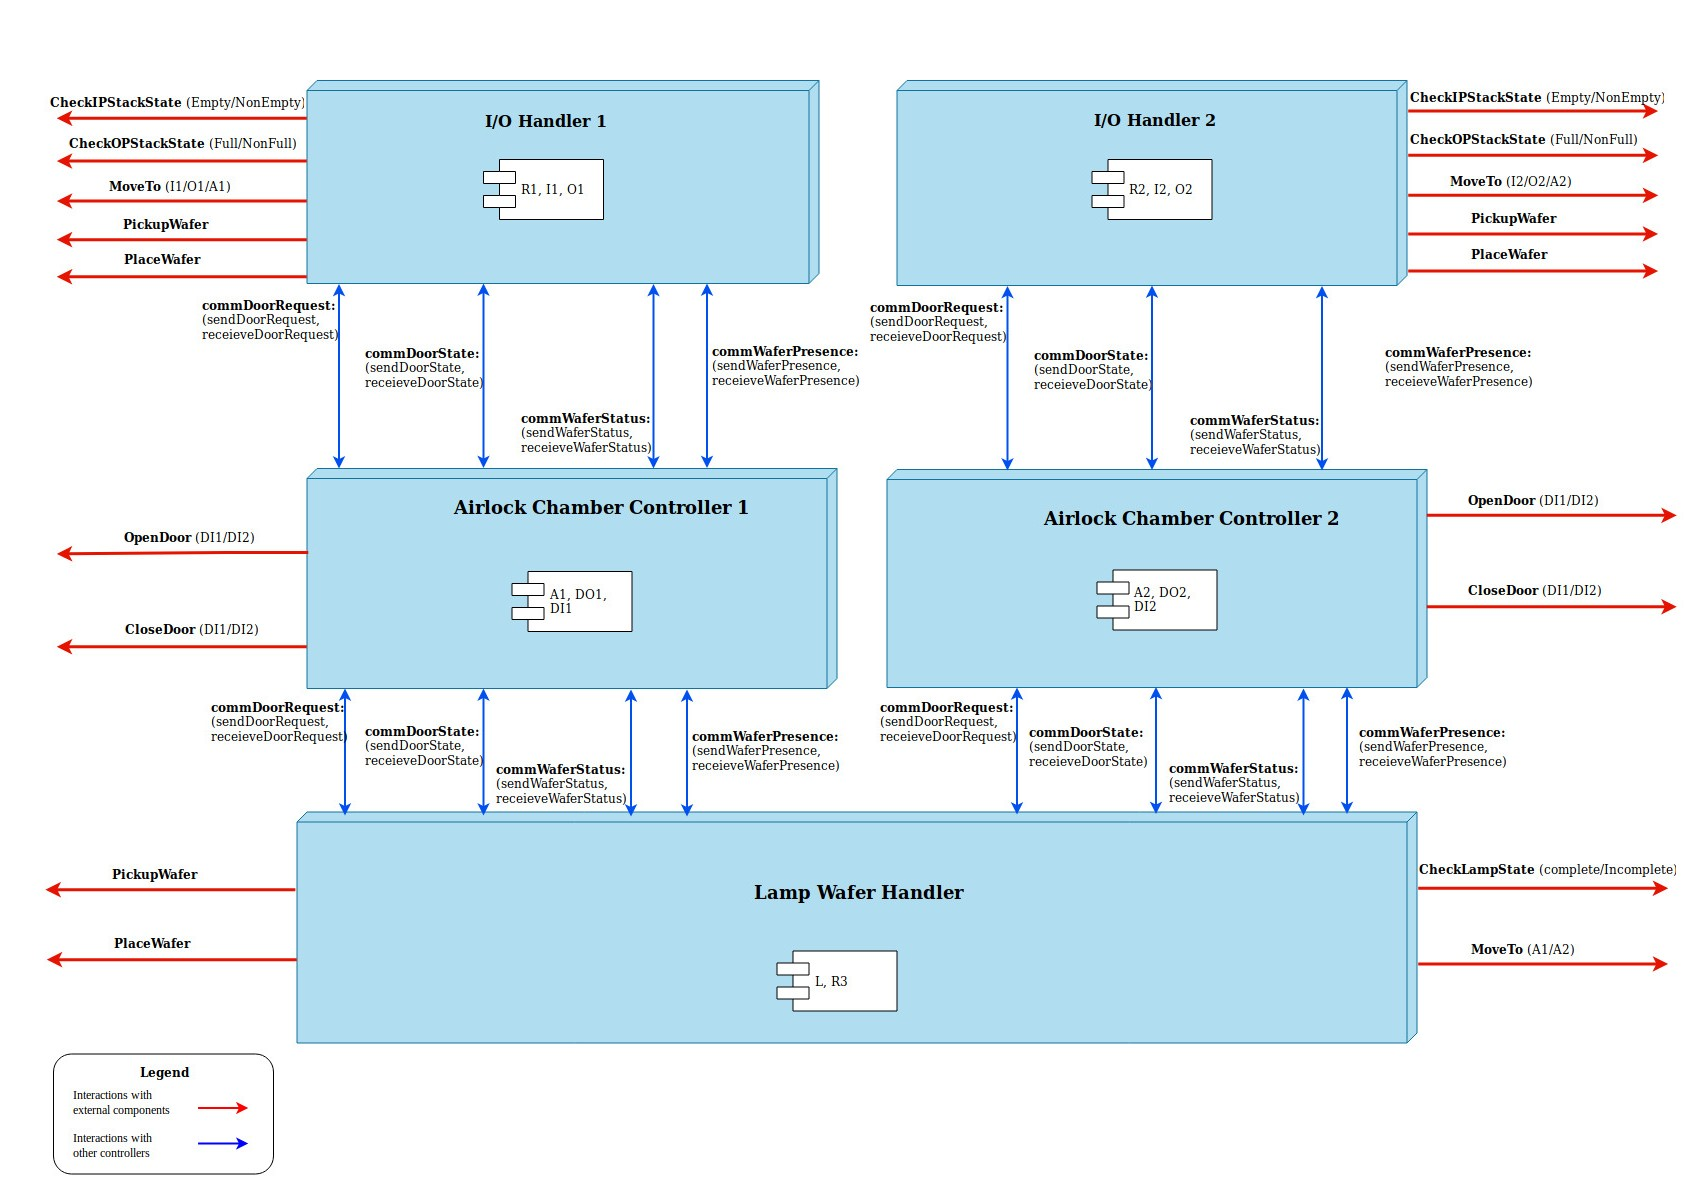
\includegraphics[width=\textwidth]{Architecture-final.jpg}
  \caption{Architecture Diagram of System}
  \label{fig:arch1}
\end{figure}
\newpage
\section{Translated Requirements}
\subsection{Introduction}
The requirements mentioned in Section 2 describe what is needed and expected out of the system. A successful verification of the system which conforms to the aforementioned specifications and requirements is to be carried out. This necessitates the use of Modal $\mu$-Calculus.   
\subsection{Modal $\mu$ -Formulas}
%\\In order to translate the requirements into their corresponding MCF representations, the requirements are rephrased as follows:
Here the corresponding Modal $\mu$ -Formulas are described:
\begin{enumerate}
\item The Robots (R1 and R2) should not move to the Input Stacks if the Input Stacks are Empty:
    \begin{itemize}
	\item MCF
	\end{itemize}
\item The Robots (R1 and R2) should not move to the Output Stacks if the Output Stacks are Full:
    \begin{itemize}
	\item MCF
	\end{itemize}
\item The Robots (R1 and R2) should not move to the Output Stacks without a finished wafer:
    \begin{itemize}
	\item MCF
	\end{itemize}
\item The Robots (R1 and R2) should not place a new wafer on the Output Stacks (O1 and O2):
    \begin{itemize}
	\item MCF
	\end{itemize}
\item The Robots (R1 and R2) should not place a wafer on the Input Stacks (I1 and I2):
    \begin{itemize}
	\item MCF
	\end{itemize}
\item The Robots (R1 and R2) should not move to the Airlocks (A1 and A2) if the corresponding Outer Doors are closed (DO1 and DO2):
    \begin{itemize}
	\item MCF
	\end{itemize}
\item The Robot (R3) should not move to the Airlocks (A1 or A2) if the corresponding Inner Doors are closed:
    \begin{itemize}
	\item MCF
	\end{itemize}
\item The Inner Door (DI1) must not be opened if the Outer Door(DO1) is open for Airlock (A1).
\item The Inner Door (DI2) must not be opened if the Outer Door(DO2) is open for Airlock (A2).
\item The Outer Door (DO1) must not be opened if the Inner Door(DI1) is open for Airlock (A1).
\item The Outer Door (DO2) must not be opened if the Inner Door(DI2) is open for Airlock (A2) :
\begin{itemize}
	\item (for 8-11) MCF
	\end{itemize}
\item The Inner Doors (DI1 and DI2) must not be opened if a finished wafer is present in their corresponding Airlocks (A1 and A2):
    \begin{itemize}
	\item MCF
	\end{itemize}
\item The Outer Doors (DO1 and DO2) must not be opened if a new wafer is present in their corresponding Airlocks (A1 and A2):
    \begin{itemize}
	\item MCF
	\end{itemize}
\item The Robot (R3) will place the new wafer on the Lamp only when it is empty:
    \begin{itemize}
	\item MCF
	\end{itemize}
\item The Robot (R3) will pickup the finished wafer from the Lamp (L) only when it is finished printing:
    \begin{itemize}
	\item MCF
	\end{itemize}
\item The Robot (R3) will not place the finished wafer again on the Lamp (L):
    \begin{itemize}
	\item MCF
	\end{itemize}
\item The Robot (R3) will not pickup a wafer immediately after it has placed a wafer:
    \begin{itemize}
	\item MCF
	\end{itemize}
\item The Robot (R3) will place a wafer it picked from an Airlock (A1 or A2) only to the same Airlock (after processing):
    \begin{itemize}
	\item MCF
	\end{itemize}
	
\end{enumerate}
\newpage
\section{Modelling the System}
Currently the two controllers called IO Handler 1 and IO Handler 2 are working in parallel with 2 separate Airlock Controllers for each Airlock and with the Lamp Handler. This results in a system with five parallel components working to move the wafer along the production process. The system currently has 87 levels, 1740 states and 3776 transitions.
\\
\\We have however, restricted the controllers to only control and interact with one half of the symmetrical system. This implies that the IO Handlers and Airlock Controllers only interact with a single robot (R1 or R2), single pair of Input and Output stack (I1,O1 or I2,O2), Airlocks (A1 or A2) and the corresponding pair of doors (DO1,DI1 or DO2,DI2). This simplifies the system to a great extent and helps in it's modelling.
\\
\\There is a caveat that this simplification will reduce the throughput of the system. This happens when one of the Stacks no longer have wafers present but the other pair of stacks still do. Hence, as an extension, we have considered the possibility of modelling a system which will have the flexibility to move the robots to different stacks and hence increase the throughput. 
\begin{figure}[ht]
\centering
    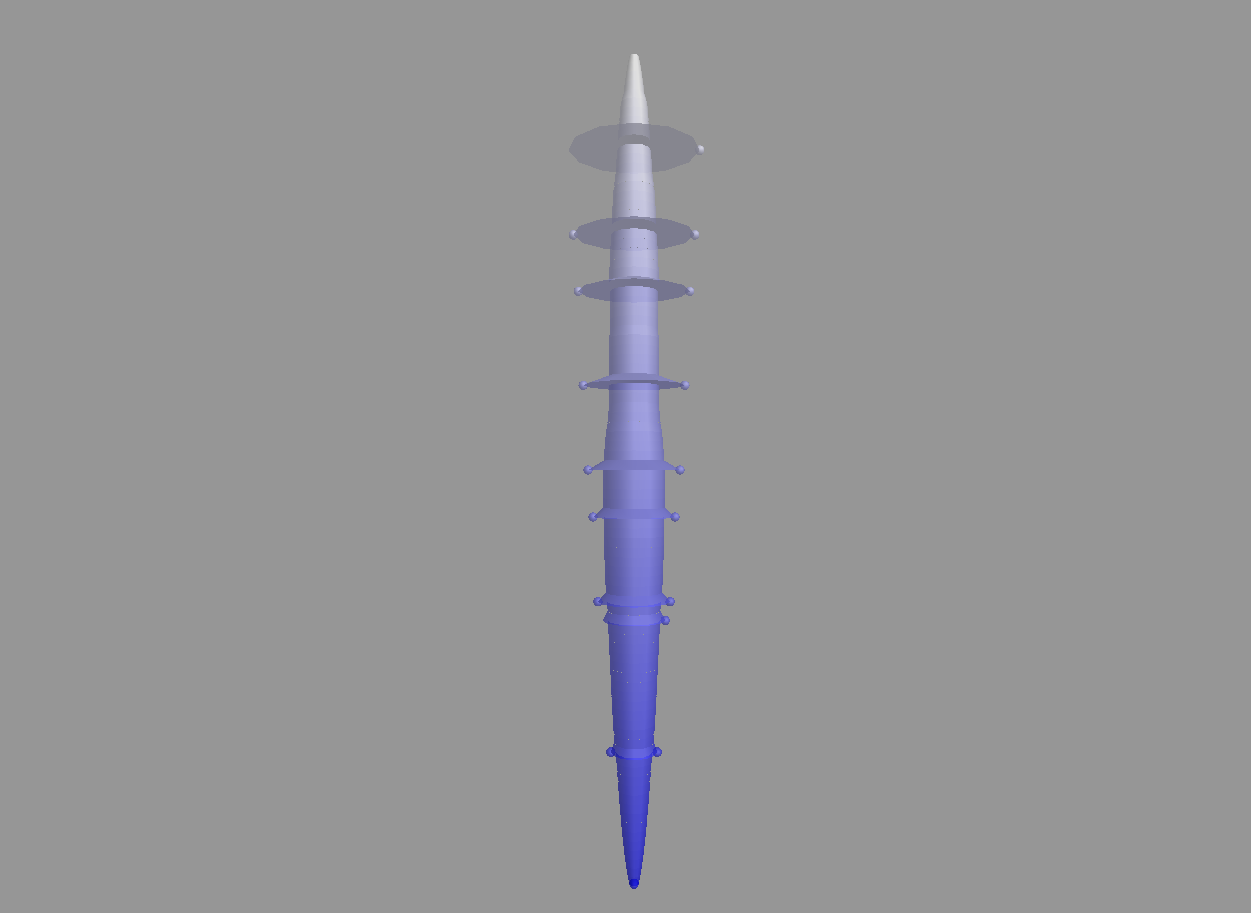
\includegraphics[width=\textwidth, height=8cm]{3D-Model.png}
  \caption{LTSView of the System}
  \label{fig:ltsview}
\end{figure}
\newpage
\section{Verification}
The Verification process involved three main steps. We created a simplified version of the model where only a single IO Handler, Airlock Controller and Lamp Handler was present. We disregarded the second pair of Input Output Stacks along with the Robot and Airlock. This way we could visualize the system using LTSGraph. This worked well because for the complete system we simply needed to extend from this simplification by doubling the number of components mentioned above. The Complete Model was visually inspected using LTSView to mark for deadlocks along with an LPSxSim simulation to logically verify the correct sequence of actions for the process. These are presented in the Visualization subsection. The $\mu$ Formulas derived from the translated requirements from Section 5 are presented in Appendix B 
\subsection{Tools}
In order to replicate our results, we provide the exact version of the tools we used along with the system configuration we used them on.
\\
\\The following version of mcrl2 was used:
\begin{itemize}
    \item mcrl2 --version: 201808.0
\end{itemize}
The following tools were used for modelling and verification:
\begin{itemize}
    \item mcrl2xi : Editing
    \item mcrl22lps : Transformation
    \item lpsxsim : Simulation
    \item lps2lts : Transformation
    \item ltsgraph : Visualization
    \item ltsview : Visualization
    \item lts2pbes : Transformation
    \item pbessolve : Verification
\end{itemize}
The following is the specification of the system used for the above tools:
\begin{itemize}
    \item Windows 10, Intel i-core i7, 2.8GHz processor with 16GB RAM 
\end{itemize}
\subsection{Verification Checks}
The method used for formal verification of the system requirements presented in Section 2 is converting the model to PBES and then verifying each MCF individually. The MCF presented in Section 5 are verified individually and each of the presented MCF holds true for the model presented.
\subsection{Visualizations}
The visual representations provide an additional guide to verify that the system is, indeed, deadlock free. Figure \ref{fig:ltsview-1} shows the system when visualized with LTSView tool. The figure represents the states and transitions present in the model. Figure \ref{fig:deadlockfree} shows the model when marked for deadlocks. The absence of red dots confirms that the system is deadlock free.
\begin{figure}[ht]
    \centering
    \begin{minipage}{0.45\textwidth}
        \centering
        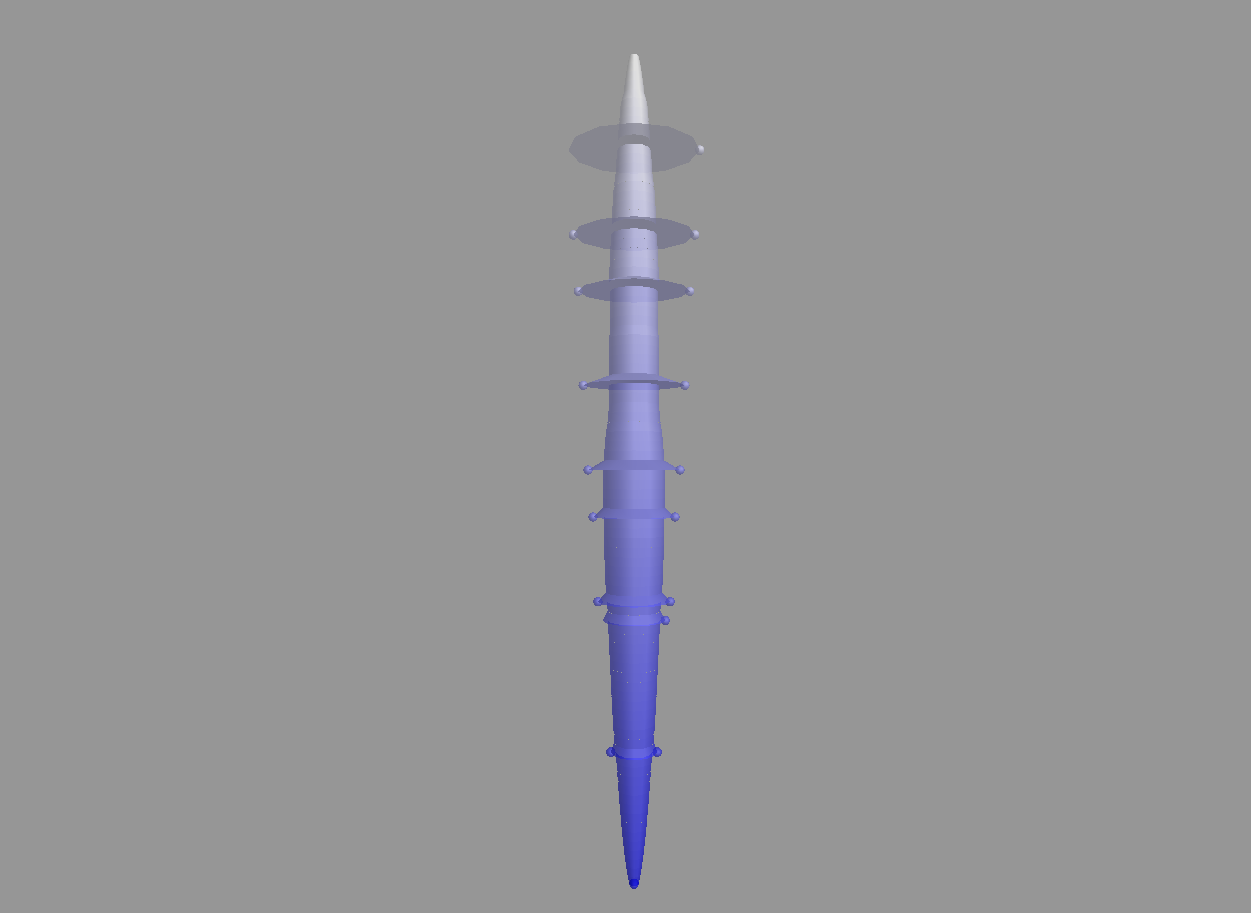
\includegraphics[width=0.9\textwidth]{3D-Model.png} \caption{LTSView}
        \label{fig:ltsview-1}
    \end{minipage}\hfill
    \begin{minipage}{0.45\textwidth}
        \centering
        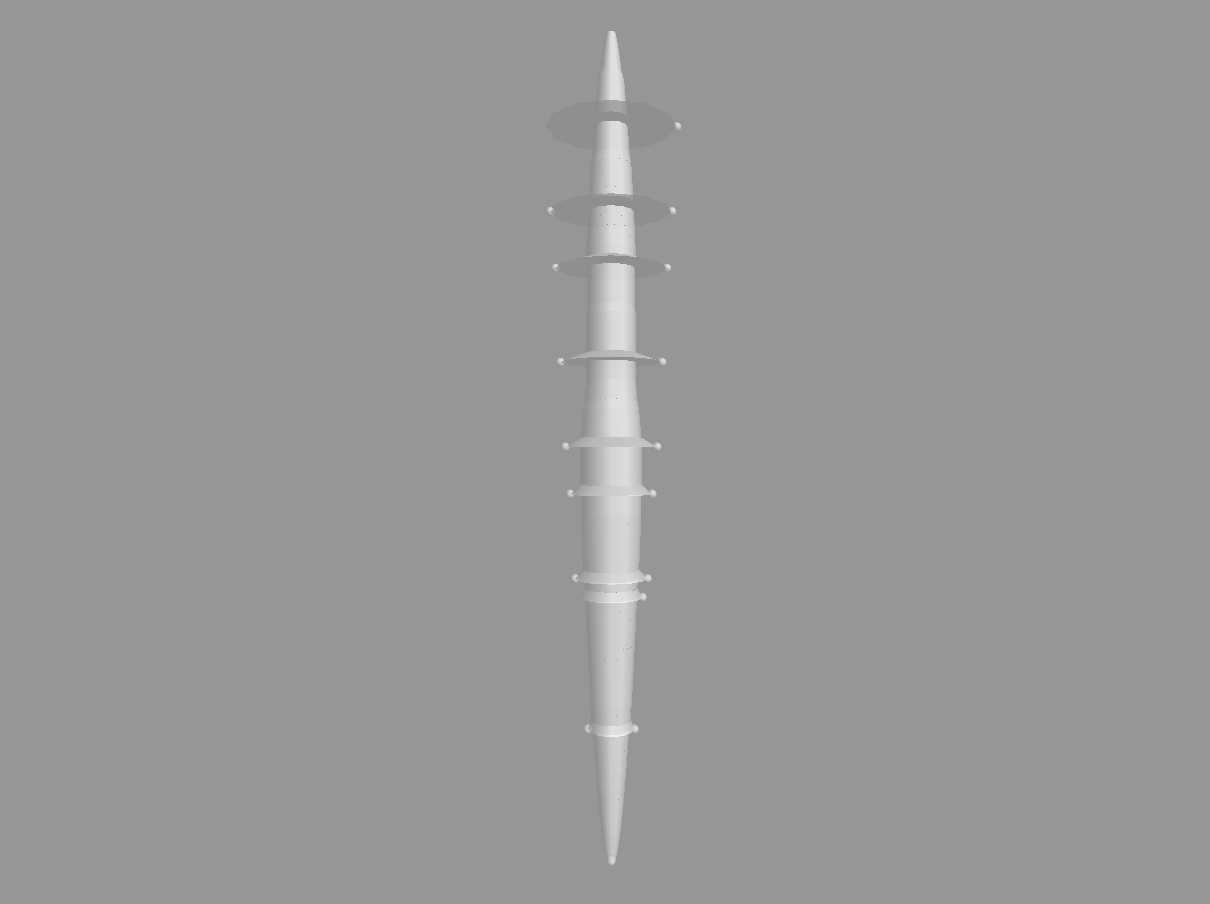
\includegraphics[width=0.9\textwidth]{Deadlockfree.png} 
        \caption{Marking Deadlocks}
        \label{fig:deadlockfree}
    \end{minipage}
\end{figure}
\section{Conclusion}
\newpage
\appendix
\section{Code: mcrl2}
\textbf{sort} DestinationID = \textbf{struct} A1 $|$ A2 $|$ I1 $|$ I2 $|$ O1 $|$ O2 $|$ Lamp;
\\		  StackID = \textbf{struct} IP1 $|$ IP2 $|$ OP1 $|$ OP2;
\\		  AirlockID = \textbf{struct} AL1 $|$ AL2 $|$ None;
\\     IOHandlerID = \textbf{struct} IOH1 $|$ IOH2;
\\		  OperationType = \textbf{struct} Get $|$ Put;
\\		  IPStackState = \textbf{struct} Empty $|$ NonEmpty;
\\		  OPStackState = \textbf{struct} Full $|$ NonFull;
\\	    DoorID = \textbf{struct} DI1 $|$ DI2 $|$ DO1 $|$ DO2;		
\\		  DoorState = \textbf{struct} Open $|$ Closed;
\\			LampState = \textbf{struct} Incomplete $|$ Complete;
\\		  CycleType = \textbf{struct} Input $|$ Output;
\\		  WaferType = \textbf{struct} New $|$ Finished $|$ NoWafer;
\\
\\\textbf{map} CorrespondingDoor : DoorID -> DoorID;
\\	  CorrespondingOPDestination : IPStackID -> \\DestinationID;		
\\	  MapOPDestination : OPStackID -> DestinationID;
\\		MapIPDestination : IPStackID -> DestinationID;
\\		MapAirlock : AirlockID -> DestinationID;
\\
\\ \textbf{eqn} CorrespondingDoor(DO1) = DI1;
\\		CorrespondingDoor(DI1) = DO1;
\\		CorrespondingDoor(DO2) = DI2;
\\		CorrespondingDoor(DI2) = DO2;
\\
\\		CorrespondingOPDestination(IP1) = O1;
\\		CorrespondingOPDestination(IP2) = O2;
\\
\\		MapOPDestination(OP1) = O1;
\\		MapOPDestination(OP2) = O2;
\\		MapIPDestination(IP1) = I1;
\\		MapIPDestination(IP2) = I2;
\\
\\		MapAirlock(AL1) = A1;
\\		MapAirlock(AL2) = A2;
\\		MapAirlock(None) = Null;
\\
\\\textbf{act} MoveTo: DestinationID;
\\	  PickupWafer;
\\	  PlaceWafer;
\\
\\	    OpenDoor : DoorID;
\\		CloseDoor : DoorID;
\\
\\	  CheckIPStackState : StackID \# IPStackState;
\\	  CheckOPStackState : StackID \# OPStackState;
\\		CheckLampState : LampState;
\\
\\	  receiveDoorState : DoorID \# DoorState;
\\	  sendDoorState : DoorID \# DoorState;
\\		commDoorState : DoorID \# DoorState;
\\
\\	  receiveDoorRequest : DoorID \# DoorState;
\\		sendDoorRequest : DoorID \# DoorState;
\\		commDoorRequest : DoorID \# DoorState;
\\
\\	  receiveWaferStatus : AirlockID \# WaferType;
\\		sendWaferStatus : AirlockID \# WaferType;
\\		commWaferStatus : AirlockID \# WaferType;
\\
\\	  receiveWaferPresence : AirlockID \# WaferType;
\\		sendWaferPresence : AirlockID \# WaferType;
\\		commWaferPresence : AirlockID \# WaferType;
\\
\\
\\\textbf{proc} IOHandler1(Operation : OperationType, Cycle : CycleType) = 
\\((Cycle == Input) \&\& (Operation == Get)) -$>$ CheckIPStackState(IP1,Empty).IOHandler1(Operation = Get)
\\+ ((Cycle == Input) \&\& (Operation == Get)) -$>$ CheckIPStackState(IP1,NonEmpty).MoveTo(I1).PickupWafer.IOHandler1(Operation = Put)
\\+ ((Cycle == Input) \&\& (Operation == Put)) -$>$ receiveDoorState(DO1,Closed).sendDoorRequest(DO1,Open).IOHandler1(Operation = Put)
\\+ ((Cycle == Input) \&\& (Operation == Put)) -$>$ receiveDoorState(DO1,Open).MoveTo(A1).PlaceWafer.sendWaferStatus(AL1,New).IOHandler1(Cycle = Output, Operation = Get)
\\
\\+ ((Cycle == Output) \&\& (Operation == Get)) -$>$ receiveWaferPresence(AL1,NoWafer).IOHandler1(Operation = Get)
\\+ ((Cycle == Output) \&\& (Operation == Get)) -$>$ receiveWaferPresence(AL1,Finished).receiveDoorState(DO1,Closed).sendDoorRequest(DO1,Open)
.receiveDoorState(DO1,Open).MoveTo(A1).PickupWafer.IOHandler1(Operation = Put)
\\
\\+ ((Cycle == Output) \&\& (Operation == Put)) -$>$ CheckOPStackState(OP1,Full).IOHandler1(Operation = Put)
\\+ ((Cycle == Output) \&\& (Operation == Put)) -$>$ CheckOPStackState(OP1,NonFull).MoveTo(O1).PlaceWafer.IOHandler1(Cycle = Input, Operation = Get);
\\
\\IOHandler2(Operation : OperationType, Cycle : CycleType) =
\\((Cycle == Input) \&\& (Operation == Get)) -$>$ CheckIPStackState(IP2,Empty).IOHandler2(Operation = Get)
\\+ ((Cycle == Input) \&\& (Operation == Get)) -$>$ CheckIPStackState(IP2,NonEmpty).MoveTo(I2).PickupWafer.IOHandler2(Operation = Put)
\\+ ((Cycle == Input) \&\& (Operation == Put)) -$>$ receiveDoorState(DO2,Closed).sendDoorRequest(DO2,Open).IOHandler2(Operation = Put)
\\+ ((Cycle == Input) \&\& (Operation == Put)) -$>$ receiveDoorState(DO2,Open).MoveTo(A2).PlaceWafer.sendWaferStatus(AL2,New).IOHandler2(Cycle = Output, Operation = Get)
\\
\\+ ((Cycle == Output) \&\& (Operation == Get)) -$>$ receiveWaferPresence(AL2,NoWafer).IOHandler2(Operation = Get)
\\+ ((Cycle == Output) \&\& (Operation == Get)) -$>$ receiveWaferPresence(AL2,Finished).receiveDoorState(DO2,Closed).sendDoorRequest(DO2,Open)
.receiveDoorState(DO2,Open).MoveTo(A2).PickupWafer.IOHandler2(Operation = Put)
\\
\\+ ((Cycle == Output) \&\& (Operation == Put)) -$>$ CheckOPStackState(OP2,Full).IOHandler2(Operation = Put)
\\+ ((Cycle == Output) \&\& (Operation == Put)) -$>$ CheckOPStackState(OP2,NonFull).MoveTo(O2).PlaceWafer.IOHandler2(Cycle = Input, Operation = Get);
\\
\\AirlockChamber1Controller(WaferPresence : WaferType, OuterDoorState : DoorState, InnerDoorState : DoorState) =
((OuterDoorState == Closed) \&\& (InnerDoorState == Open)) -$>$ receiveDoorRequest(DO1,Open).AirlockChamber1Controller(InnerDoorState = Open)
\\
\\+ ((OuterDoorState == Closed) \&\& (InnerDoorState == Closed)) -$>$ receiveDoorRequest(DO1,Open).OpenDoor(DO1).AirlockChamber1Controller(OuterDoorState = Open)
\\+ ((OuterDoorState == Open) \&\& (InnerDoorState == Closed)) -$>$ receiveDoorRequest(DI1,Open).AirlockChamber1Controller(OuterDoorState = Open)
\\+ ((OuterDoorState == Closed) \&\& (InnerDoorState == Closed)) -$>$ receiveDoorRequest(DI1,Open).OpenDoor(DI1).AirlockChamber1Controller(InnerDoorState = Open)
\\
\\+ ((OuterDoorState == Open) \&\& (InnerDoorState == Closed)) -$>$ receiveWaferStatus(AL1,New).CloseDoor(DO1).AirlockChamber1Controller(WaferPresence = New, OuterDoorState = Closed)
\\+ ((OuterDoorState == Closed) \&\& (InnerDoorState == Open)) -$>$ receiveWaferStatus(AL1,Finished).CloseDoor(DI1).AirlockChamber1Controller(WaferPresence = Finished, InnerDoorState = Closed)
\\
\\+ sendDoorState(DO1,OuterDoorState).AirlockChamber1Controller()
\\+ sendDoorState(DI1,InnerDoorState).AirlockChamber1Controller()
\\+ sendWaferPresence(AL1,WaferPresence).AirlockChamber1Controller();
\\
\\AirlockChamber2Controller(WaferPresence : WaferType, OuterDoorState : DoorState, InnerDoorState : DoorState) =
((OuterDoorState == Closed) \&\& (InnerDoorState == Open)) -$>$ receiveDoorRequest(DO2,Open).AirlockChamber2Controller(InnerDoorState = Open)
\\+ ((OuterDoorState == Closed) \&\& (InnerDoorState == Closed)) -$>$ receiveDoorRequest(DO2,Open).OpenDoor(DO2).AirlockChamber2Controller(OuterDoorState = Open)
\\+ ((OuterDoorState == Open) \&\& (InnerDoorState == Closed)) -$>$ receiveDoorRequest(DI2,Open).AirlockChamber2Controller(OuterDoorState = Open)
\\+ ((OuterDoorState == Closed) \&\& (InnerDoorState == Closed)) -$>$ receiveDoorRequest(DI2,Open).OpenDoor(DI2).AirlockChamber2Controller(InnerDoorState = Open)
\\
\\+ ((OuterDoorState == Open) \&\& (InnerDoorState == Closed)) -$>$ receiveWaferStatus(AL2,New).CloseDoor(DO2).AirlockChamber2Controller(WaferPresence = New, OuterDoorState = Closed)
\\+ ((OuterDoorState == Closed) \&\& (InnerDoorState == Open)) -$>$ receiveWaferStatus(AL2,Finished).CloseDoor(DI2).AirlockChamber2Controller(WaferPresence = Finished, InnerDoorState = Closed)
\\
\\+ sendDoorState(DO2,OuterDoorState).AirlockChamber2Controller()
\\+ sendDoorState(DI2,InnerDoorState).AirlockChamber2Controller()
\\+ sendWaferPresence(AL2,WaferPresence).AirlockChamber2Controller();
\\
\\LampWaferHandler(Cycle : CycleType, CurrentAirlock : AirlockID) = 
\\
\\((Cycle == Input) \&\& (CurrentAirlock == None)) -$>$ receiveWaferPresence(AL1,New).LampWaferHandler(CurrentAirlock = AL1)
\\+ ((Cycle == Input) \&\& (CurrentAirlock == AL1)) -$>$ receiveDoorState(DI1,Closed).sendDoorRequest(DI1,Open).LampWaferHandler(CurrentAirlock = AL1)
\\+ ((Cycle == Input) \&\& (CurrentAirlock == AL1)) -$>$ receiveDoorState(DI1,Open).MoveTo(A1).PickupWafer.MoveTo(Lamp).PlaceWafer.LampWaferHandler(Cycle = Output)
\\
\\+ ((Cycle == Output) \&\& (CurrentAirlock == AL1)) -$>$ CheckLampState(Incomplete).LampWaferHandler(Cycle = Output)
\\
\\+ ((Cycle == Output) \&\& (CurrentAirlock == AL1)) -$>$ CheckLampState(Complete).MoveTo(Lamp).PickupWafer.MoveTo(A1).PlaceWafer.sendWaferStatus(AL1,Finished).LampWaferHandler(Cycle = Input, CurrentAirlock = None)
\\
\\+ ((Cycle == Input) \&\& (CurrentAirlock == None)) -$>$ receiveWaferPresence(AL2,New).LampWaferHandler(CurrentAirlock = AL2)
\\
\\+ ((Cycle == Input) \&\& (CurrentAirlock == AL2)) -$>$ receiveDoorState(DI2,Closed).sendDoorRequest(DI2,Open).LampWaferHandler(CurrentAirlock = AL2)
\\
\\+ ((Cycle == Input) \&\& (CurrentAirlock == AL2)) -$>$ receiveDoorState(DI2,Open).MoveTo(A2).PickupWafer.MoveTo(Lamp).PlaceWafer.LampWaferHandler(Cycle = Output)
\\
\\+ ((Cycle == Output) \&\& (CurrentAirlock == AL2)) -$>$ CheckLampState(Incomplete).LampWaferHandler(Cycle = Output)
\\
\\+ ((Cycle == Output) \&\& (CurrentAirlock == AL2)) -$>$ CheckLampState(Complete).MoveTo(Lamp).PickupWafer.MoveTo(A2).PlaceWafer.sendWaferStatus(AL2,Finished).LampWaferHandler(Cycle = Input, CurrentAirlock = None);
\\
\\\textbf{init} 
\\
\\\textbf{			allow}(
\\						{MoveTo,
 \\ 				 	 PickupWafer,
 \\				 		 PlaceWafer,
 \\	    			 CheckIPStackState,
\\	  				 CheckOPStackState,
\\						 CheckLampState,
\\						 OpenDoor,
\\						 CloseDoor,
\\
\\						 commDoorState,
\\						 commDoorRequest,
\\						 commWaferStatus,
\\						 commWaferPresence},
\\
\\\textbf{			comm}(
\\						{receiveDoorState $|$ sendDoorState -$>$ commDoorState,
\\						receiveDoorRequest $|$ sendDoorRequest -$>$ commDoorRequest,
\\	  				 	receiveWaferStatus $|$ sendWaferStatus -$>$ commWaferStatus,
\\				 	   receiveWaferPresence $|$ sendWaferPresence -$>$ commWaferPresence},
\\
\\						 IOHandler1(Get, Input) $|$ $|$ IOHandler2(Get, Input) $|$ $|$ AirlockChamber1Controller(NoWafer, Closed, Closed) $|$ $|$ AirlockChamber2Controller(NoWafer, Closed, Closed) $|$ $|$ LampWaferHandler(Input,None)
\\					 ));
\newpage
\section{Code: $\mu$-Formulas}

\end{document}
